\documentclass[12pt]{article}
\renewcommand{\thesection}{\Roman{section}} 
\renewcommand{\thesubsection}{\thesection.\Roman{subsection}}
\usepackage[tocindentauto]{tocstyle}
%\usetocstyle{KOMAlike} %the previous line resets it
\usepackage{natbib}
\usepackage{url}
\usepackage[utf8x]{inputenc}
\usepackage{amsmath}
\usepackage{graphicx}
\usepackage[demo]{graphicx}
\usepackage{verbatim}
\graphicspath{{images/}}
\usepackage{parskip}
\usepackage{fancyhdr}
\usepackage{vmargin}
\setmarginsrb{3 cm}{2.5 cm}{3 cm}{2.5 cm}{1 cm}{1.5 cm}{1 cm}{1.5 cm}
\usepackage{appendix}
\usepackage{listings} % For code importing
\usepackage{xcolor} % for setting colors
 %%%%%%%%%%%%%%%%%%%%%%%%%%%%%%%%%%%%%%%%%%%%%%%%%%%%%%%%%%%%%%%%%%%%%%%%%%%%%%%% 
%%% ~ Arduino Language - Arduino IDE Colors ~                                  %%%
%%%                                                                            %%%
%%% Kyle Rocha-Brownell | 10/2/2017 | No Licence                               %%%
%%% -------------------------------------------------------------------------- %%%
%%%                                                                            %%%
%%% Place this file in your working directory (next to the latex file you're   %%%
%%% working on).  To add it to your project, place:                            %%%
%%%     %%%%%%%%%%%%%%%%%%%%%%%%%%%%%%%%%%%%%%%%%%%%%%%%%%%%%%%%%%%%%%%%%%%%%%%%%%%%%%%% 
%%% ~ Arduino Language - Arduino IDE Colors ~                                  %%%
%%%                                                                            %%%
%%% Kyle Rocha-Brownell | 10/2/2017 | No Licence                               %%%
%%% -------------------------------------------------------------------------- %%%
%%%                                                                            %%%
%%% Place this file in your working directory (next to the latex file you're   %%%
%%% working on).  To add it to your project, place:                            %%%
%%%     %%%%%%%%%%%%%%%%%%%%%%%%%%%%%%%%%%%%%%%%%%%%%%%%%%%%%%%%%%%%%%%%%%%%%%%%%%%%%%%% 
%%% ~ Arduino Language - Arduino IDE Colors ~                                  %%%
%%%                                                                            %%%
%%% Kyle Rocha-Brownell | 10/2/2017 | No Licence                               %%%
%%% -------------------------------------------------------------------------- %%%
%%%                                                                            %%%
%%% Place this file in your working directory (next to the latex file you're   %%%
%%% working on).  To add it to your project, place:                            %%%
%%%    \input{arduinoLanguage.tex}                                             %%%
%%% somewhere before \begin{document} in your latex file.                      %%%
%%%                                                                            %%%
%%% In your document, place your arduino code between:                         %%%
%%%   \begin{lstlisting}[language=Arduino]                                     %%%
%%% and:                                                                       %%%
%%%   \end{lstlisting}                                                         %%%
%%%                                                                            %%%
%%% Or create your own style to add non-built-in functions and variables.      %%%
%%%                                                                            %%%
 %%%%%%%%%%%%%%%%%%%%%%%%%%%%%%%%%%%%%%%%%%%%%%%%%%%%%%%%%%%%%%%%%%%%%%%%%%%%%%%% 

\usepackage{color}
\usepackage{listings}    
\usepackage{courier}

%%% Define Custom IDE Colors %%%
\definecolor{arduinoGreen}    {rgb} {0.17, 0.43, 0.01}
\definecolor{arduinoGrey}     {rgb} {0.47, 0.47, 0.33}
\definecolor{arduinoOrange}   {rgb} {0.8 , 0.4 , 0   }
\definecolor{arduinoBlue}     {rgb} {0.01, 0.61, 0.98}
\definecolor{arduinoDarkBlue} {rgb} {0.0 , 0.2 , 0.5 }

%%% Define Arduino Language %%%
\lstdefinelanguage{Arduino}{
  language=C++, % begin with default C++ settings 
%
%
  %%% Keyword Color Group 1 %%%  (called KEYWORD3 by arduino)
  keywordstyle=\color{arduinoGreen},   
  deletekeywords={  % remove all arduino keywords that might be in c++
                break, case, override, final, continue, default, do, else, for, 
                if, return, goto, switch, throw, try, while, setup, loop, export, 
                not, or, and, xor, include, define, elif, else, error, if, ifdef, 
                ifndef, pragma, warning,
                HIGH, LOW, INPUT, INPUT_PULLUP, OUTPUT, DEC, BIN, HEX, OCT, PI, 
                HALF_PI, TWO_PI, LSBFIRST, MSBFIRST, CHANGE, FALLING, RISING, 
                DEFAULT, EXTERNAL, INTERNAL, INTERNAL1V1, INTERNAL2V56, LED_BUILTIN, 
                LED_BUILTIN_RX, LED_BUILTIN_TX, DIGITAL_MESSAGE, FIRMATA_STRING, 
                ANALOG_MESSAGE, REPORT_DIGITAL, REPORT_ANALOG, SET_PIN_MODE, 
                SYSTEM_RESET, SYSEX_START, auto, int8_t, int16_t, int32_t, int64_t, 
                uint8_t, uint16_t, uint32_t, uint64_t, char16_t, char32_t, operator, 
                enum, delete, bool, boolean, byte, char, const, false, float, double, 
                null, NULL, int, long, new, private, protected, public, short, 
                signed, static, volatile, String, void, true, unsigned, word, array, 
                sizeof, dynamic_cast, typedef, const_cast, struct, static_cast, union, 
                friend, extern, class, reinterpret_cast, register, explicit, inline, 
                _Bool, complex, _Complex, _Imaginary, atomic_bool, atomic_char, 
                atomic_schar, atomic_uchar, atomic_short, atomic_ushort, atomic_int, 
                atomic_uint, atomic_long, atomic_ulong, atomic_llong, atomic_ullong, 
                virtual, PROGMEM,
                Serial, Serial1, Serial2, Serial3, SerialUSB, Keyboard, Mouse,
                abs, acos, asin, atan, atan2, ceil, constrain, cos, degrees, exp, 
                floor, log, map, max, min, radians, random, randomSeed, round, sin, 
                sq, sqrt, tan, pow, bitRead, bitWrite, bitSet, bitClear, bit, 
                highByte, lowByte, analogReference, analogRead, 
                analogReadResolution, analogWrite, analogWriteResolution, 
                attachInterrupt, detachInterrupt, digitalPinToInterrupt, delay, 
                delayMicroseconds, digitalWrite, digitalRead, interrupts, millis, 
                micros, noInterrupts, noTone, pinMode, pulseIn, pulseInLong, shiftIn, 
                shiftOut, tone, yield, Stream, begin, end, peek, read, print, 
                println, available, availableForWrite, flush, setTimeout, find, 
                findUntil, parseInt, parseFloat, readBytes, readBytesUntil, readString, 
                readStringUntil, trim, toUpperCase, toLowerCase, charAt, compareTo, 
                concat, endsWith, startsWith, equals, equalsIgnoreCase, getBytes, 
                indexOf, lastIndexOf, length, replace, setCharAt, substring, 
                toCharArray, toInt, press, release, releaseAll, accept, click, move, 
                isPressed, isAlphaNumeric, isAlpha, isAscii, isWhitespace, isControl, 
                isDigit, isGraph, isLowerCase, isPrintable, isPunct, isSpace, 
                isUpperCase, isHexadecimalDigit, 
                }, 
  morekeywords={   % add arduino structures to group 1
                break, case, override, final, continue, default, do, else, for, 
                if, return, goto, switch, throw, try, while, setup, loop, export, 
                not, or, and, xor, include, define, elif, else, error, if, ifdef, 
                ifndef, pragma, warning,
                }, 
% 
%
  %%% Keyword Color Group 2 %%%  (called LITERAL1 by arduino)
  keywordstyle=[2]\color{arduinoBlue},   
  keywords=[2]{   % add variables and dataTypes as 2nd group  
                HIGH, LOW, INPUT, INPUT_PULLUP, OUTPUT, DEC, BIN, HEX, OCT, PI, 
                HALF_PI, TWO_PI, LSBFIRST, MSBFIRST, CHANGE, FALLING, RISING, 
                DEFAULT, EXTERNAL, INTERNAL, INTERNAL1V1, INTERNAL2V56, LED_BUILTIN, 
                LED_BUILTIN_RX, LED_BUILTIN_TX, DIGITAL_MESSAGE, FIRMATA_STRING, 
                ANALOG_MESSAGE, REPORT_DIGITAL, REPORT_ANALOG, SET_PIN_MODE, 
                SYSTEM_RESET, SYSEX_START, auto, int8_t, int16_t, int32_t, int64_t, 
                uint8_t, uint16_t, uint32_t, uint64_t, char16_t, char32_t, operator, 
                enum, delete, bool, boolean, byte, char, const, false, float, double, 
                null, NULL, int, long, new, private, protected, public, short, 
                signed, static, volatile, String, void, true, unsigned, word, array, 
                sizeof, dynamic_cast, typedef, const_cast, struct, static_cast, union, 
                friend, extern, class, reinterpret_cast, register, explicit, inline, 
                _Bool, complex, _Complex, _Imaginary, atomic_bool, atomic_char, 
                atomic_schar, atomic_uchar, atomic_short, atomic_ushort, atomic_int, 
                atomic_uint, atomic_long, atomic_ulong, atomic_llong, atomic_ullong, 
                virtual, PROGMEM,
                },  
% 
%
  %%% Keyword Color Group 3 %%%  (called KEYWORD1 by arduino)
  keywordstyle=[3]\bfseries\color{arduinoOrange},
  keywords=[3]{  % add built-in functions as a 3rd group
                Serial, Serial1, Serial2, Serial3, SerialUSB, Keyboard, Mouse,
                },      
%
%
  %%% Keyword Color Group 4 %%%  (called KEYWORD2 by arduino)
  keywordstyle=[4]\color{arduinoOrange},
  keywords=[4]{  % add more built-in functions as a 4th group
                abs, acos, asin, atan, atan2, ceil, constrain, cos, degrees, exp, 
                floor, log, map, max, min, radians, random, randomSeed, round, sin, 
                sq, sqrt, tan, pow, bitRead, bitWrite, bitSet, bitClear, bit, 
                highByte, lowByte, analogReference, analogRead, 
                analogReadResolution, analogWrite, analogWriteResolution, 
                attachInterrupt, detachInterrupt, digitalPinToInterrupt, delay, 
                delayMicroseconds, digitalWrite, digitalRead, interrupts, millis, 
                micros, noInterrupts, noTone, pinMode, pulseIn, pulseInLong, shiftIn, 
                shiftOut, tone, yield, Stream, begin, end, peek, read, print, 
                println, available, availableForWrite, flush, setTimeout, find, 
                findUntil, parseInt, parseFloat, readBytes, readBytesUntil, readString, 
                readStringUntil, trim, toUpperCase, toLowerCase, charAt, compareTo, 
                concat, endsWith, startsWith, equals, equalsIgnoreCase, getBytes, 
                indexOf, lastIndexOf, length, replace, setCharAt, substring, 
                toCharArray, toInt, press, release, releaseAll, accept, click, move, 
                isPressed, isAlphaNumeric, isAlpha, isAscii, isWhitespace, isControl, 
                isDigit, isGraph, isLowerCase, isPrintable, isPunct, isSpace, 
                isUpperCase, isHexadecimalDigit, 
                },      
%
%
  %%% Set Other Colors %%%
  stringstyle=\color{arduinoDarkBlue},    
  commentstyle=\color{arduinoGrey},    
%          
%   
  %%%% Line Numbering %%%%
   numbers=left,                    
  numbersep=5pt,                   
  numberstyle=\color{arduinoGrey},    
  %stepnumber=2,                      % show every 2 line numbers
%
%
  %%%% Code Box Style %%%%
  breaklines=true,                    % wordwrapping
  tabsize=2,         
  basicstyle=\ttfamily  
}                                             %%%
%%% somewhere before \begin{document} in your latex file.                      %%%
%%%                                                                            %%%
%%% In your document, place your arduino code between:                         %%%
%%%   \begin{lstlisting}[language=Arduino]                                     %%%
%%% and:                                                                       %%%
%%%   \end{lstlisting}                                                         %%%
%%%                                                                            %%%
%%% Or create your own style to add non-built-in functions and variables.      %%%
%%%                                                                            %%%
 %%%%%%%%%%%%%%%%%%%%%%%%%%%%%%%%%%%%%%%%%%%%%%%%%%%%%%%%%%%%%%%%%%%%%%%%%%%%%%%% 

\usepackage{color}
\usepackage{listings}    
\usepackage{courier}

%%% Define Custom IDE Colors %%%
\definecolor{arduinoGreen}    {rgb} {0.17, 0.43, 0.01}
\definecolor{arduinoGrey}     {rgb} {0.47, 0.47, 0.33}
\definecolor{arduinoOrange}   {rgb} {0.8 , 0.4 , 0   }
\definecolor{arduinoBlue}     {rgb} {0.01, 0.61, 0.98}
\definecolor{arduinoDarkBlue} {rgb} {0.0 , 0.2 , 0.5 }

%%% Define Arduino Language %%%
\lstdefinelanguage{Arduino}{
  language=C++, % begin with default C++ settings 
%
%
  %%% Keyword Color Group 1 %%%  (called KEYWORD3 by arduino)
  keywordstyle=\color{arduinoGreen},   
  deletekeywords={  % remove all arduino keywords that might be in c++
                break, case, override, final, continue, default, do, else, for, 
                if, return, goto, switch, throw, try, while, setup, loop, export, 
                not, or, and, xor, include, define, elif, else, error, if, ifdef, 
                ifndef, pragma, warning,
                HIGH, LOW, INPUT, INPUT_PULLUP, OUTPUT, DEC, BIN, HEX, OCT, PI, 
                HALF_PI, TWO_PI, LSBFIRST, MSBFIRST, CHANGE, FALLING, RISING, 
                DEFAULT, EXTERNAL, INTERNAL, INTERNAL1V1, INTERNAL2V56, LED_BUILTIN, 
                LED_BUILTIN_RX, LED_BUILTIN_TX, DIGITAL_MESSAGE, FIRMATA_STRING, 
                ANALOG_MESSAGE, REPORT_DIGITAL, REPORT_ANALOG, SET_PIN_MODE, 
                SYSTEM_RESET, SYSEX_START, auto, int8_t, int16_t, int32_t, int64_t, 
                uint8_t, uint16_t, uint32_t, uint64_t, char16_t, char32_t, operator, 
                enum, delete, bool, boolean, byte, char, const, false, float, double, 
                null, NULL, int, long, new, private, protected, public, short, 
                signed, static, volatile, String, void, true, unsigned, word, array, 
                sizeof, dynamic_cast, typedef, const_cast, struct, static_cast, union, 
                friend, extern, class, reinterpret_cast, register, explicit, inline, 
                _Bool, complex, _Complex, _Imaginary, atomic_bool, atomic_char, 
                atomic_schar, atomic_uchar, atomic_short, atomic_ushort, atomic_int, 
                atomic_uint, atomic_long, atomic_ulong, atomic_llong, atomic_ullong, 
                virtual, PROGMEM,
                Serial, Serial1, Serial2, Serial3, SerialUSB, Keyboard, Mouse,
                abs, acos, asin, atan, atan2, ceil, constrain, cos, degrees, exp, 
                floor, log, map, max, min, radians, random, randomSeed, round, sin, 
                sq, sqrt, tan, pow, bitRead, bitWrite, bitSet, bitClear, bit, 
                highByte, lowByte, analogReference, analogRead, 
                analogReadResolution, analogWrite, analogWriteResolution, 
                attachInterrupt, detachInterrupt, digitalPinToInterrupt, delay, 
                delayMicroseconds, digitalWrite, digitalRead, interrupts, millis, 
                micros, noInterrupts, noTone, pinMode, pulseIn, pulseInLong, shiftIn, 
                shiftOut, tone, yield, Stream, begin, end, peek, read, print, 
                println, available, availableForWrite, flush, setTimeout, find, 
                findUntil, parseInt, parseFloat, readBytes, readBytesUntil, readString, 
                readStringUntil, trim, toUpperCase, toLowerCase, charAt, compareTo, 
                concat, endsWith, startsWith, equals, equalsIgnoreCase, getBytes, 
                indexOf, lastIndexOf, length, replace, setCharAt, substring, 
                toCharArray, toInt, press, release, releaseAll, accept, click, move, 
                isPressed, isAlphaNumeric, isAlpha, isAscii, isWhitespace, isControl, 
                isDigit, isGraph, isLowerCase, isPrintable, isPunct, isSpace, 
                isUpperCase, isHexadecimalDigit, 
                }, 
  morekeywords={   % add arduino structures to group 1
                break, case, override, final, continue, default, do, else, for, 
                if, return, goto, switch, throw, try, while, setup, loop, export, 
                not, or, and, xor, include, define, elif, else, error, if, ifdef, 
                ifndef, pragma, warning,
                }, 
% 
%
  %%% Keyword Color Group 2 %%%  (called LITERAL1 by arduino)
  keywordstyle=[2]\color{arduinoBlue},   
  keywords=[2]{   % add variables and dataTypes as 2nd group  
                HIGH, LOW, INPUT, INPUT_PULLUP, OUTPUT, DEC, BIN, HEX, OCT, PI, 
                HALF_PI, TWO_PI, LSBFIRST, MSBFIRST, CHANGE, FALLING, RISING, 
                DEFAULT, EXTERNAL, INTERNAL, INTERNAL1V1, INTERNAL2V56, LED_BUILTIN, 
                LED_BUILTIN_RX, LED_BUILTIN_TX, DIGITAL_MESSAGE, FIRMATA_STRING, 
                ANALOG_MESSAGE, REPORT_DIGITAL, REPORT_ANALOG, SET_PIN_MODE, 
                SYSTEM_RESET, SYSEX_START, auto, int8_t, int16_t, int32_t, int64_t, 
                uint8_t, uint16_t, uint32_t, uint64_t, char16_t, char32_t, operator, 
                enum, delete, bool, boolean, byte, char, const, false, float, double, 
                null, NULL, int, long, new, private, protected, public, short, 
                signed, static, volatile, String, void, true, unsigned, word, array, 
                sizeof, dynamic_cast, typedef, const_cast, struct, static_cast, union, 
                friend, extern, class, reinterpret_cast, register, explicit, inline, 
                _Bool, complex, _Complex, _Imaginary, atomic_bool, atomic_char, 
                atomic_schar, atomic_uchar, atomic_short, atomic_ushort, atomic_int, 
                atomic_uint, atomic_long, atomic_ulong, atomic_llong, atomic_ullong, 
                virtual, PROGMEM,
                },  
% 
%
  %%% Keyword Color Group 3 %%%  (called KEYWORD1 by arduino)
  keywordstyle=[3]\bfseries\color{arduinoOrange},
  keywords=[3]{  % add built-in functions as a 3rd group
                Serial, Serial1, Serial2, Serial3, SerialUSB, Keyboard, Mouse,
                },      
%
%
  %%% Keyword Color Group 4 %%%  (called KEYWORD2 by arduino)
  keywordstyle=[4]\color{arduinoOrange},
  keywords=[4]{  % add more built-in functions as a 4th group
                abs, acos, asin, atan, atan2, ceil, constrain, cos, degrees, exp, 
                floor, log, map, max, min, radians, random, randomSeed, round, sin, 
                sq, sqrt, tan, pow, bitRead, bitWrite, bitSet, bitClear, bit, 
                highByte, lowByte, analogReference, analogRead, 
                analogReadResolution, analogWrite, analogWriteResolution, 
                attachInterrupt, detachInterrupt, digitalPinToInterrupt, delay, 
                delayMicroseconds, digitalWrite, digitalRead, interrupts, millis, 
                micros, noInterrupts, noTone, pinMode, pulseIn, pulseInLong, shiftIn, 
                shiftOut, tone, yield, Stream, begin, end, peek, read, print, 
                println, available, availableForWrite, flush, setTimeout, find, 
                findUntil, parseInt, parseFloat, readBytes, readBytesUntil, readString, 
                readStringUntil, trim, toUpperCase, toLowerCase, charAt, compareTo, 
                concat, endsWith, startsWith, equals, equalsIgnoreCase, getBytes, 
                indexOf, lastIndexOf, length, replace, setCharAt, substring, 
                toCharArray, toInt, press, release, releaseAll, accept, click, move, 
                isPressed, isAlphaNumeric, isAlpha, isAscii, isWhitespace, isControl, 
                isDigit, isGraph, isLowerCase, isPrintable, isPunct, isSpace, 
                isUpperCase, isHexadecimalDigit, 
                },      
%
%
  %%% Set Other Colors %%%
  stringstyle=\color{arduinoDarkBlue},    
  commentstyle=\color{arduinoGrey},    
%          
%   
  %%%% Line Numbering %%%%
   numbers=left,                    
  numbersep=5pt,                   
  numberstyle=\color{arduinoGrey},    
  %stepnumber=2,                      % show every 2 line numbers
%
%
  %%%% Code Box Style %%%%
  breaklines=true,                    % wordwrapping
  tabsize=2,         
  basicstyle=\ttfamily  
}                                             %%%
%%% somewhere before \begin{document} in your latex file.                      %%%
%%%                                                                            %%%
%%% In your document, place your arduino code between:                         %%%
%%%   \begin{lstlisting}[language=Arduino]                                     %%%
%%% and:                                                                       %%%
%%%   \end{lstlisting}                                                         %%%
%%%                                                                            %%%
%%% Or create your own style to add non-built-in functions and variables.      %%%
%%%                                                                            %%%
 %%%%%%%%%%%%%%%%%%%%%%%%%%%%%%%%%%%%%%%%%%%%%%%%%%%%%%%%%%%%%%%%%%%%%%%%%%%%%%%% 

\usepackage{color}
\usepackage{listings}    
\usepackage{courier}

%%% Define Custom IDE Colors %%%
\definecolor{arduinoGreen}    {rgb} {0.17, 0.43, 0.01}
\definecolor{arduinoGrey}     {rgb} {0.47, 0.47, 0.33}
\definecolor{arduinoOrange}   {rgb} {0.8 , 0.4 , 0   }
\definecolor{arduinoBlue}     {rgb} {0.01, 0.61, 0.98}
\definecolor{arduinoDarkBlue} {rgb} {0.0 , 0.2 , 0.5 }

%%% Define Arduino Language %%%
\lstdefinelanguage{Arduino}{
  language=C++, % begin with default C++ settings 
%
%
  %%% Keyword Color Group 1 %%%  (called KEYWORD3 by arduino)
  keywordstyle=\color{arduinoGreen},   
  deletekeywords={  % remove all arduino keywords that might be in c++
                break, case, override, final, continue, default, do, else, for, 
                if, return, goto, switch, throw, try, while, setup, loop, export, 
                not, or, and, xor, include, define, elif, else, error, if, ifdef, 
                ifndef, pragma, warning,
                HIGH, LOW, INPUT, INPUT_PULLUP, OUTPUT, DEC, BIN, HEX, OCT, PI, 
                HALF_PI, TWO_PI, LSBFIRST, MSBFIRST, CHANGE, FALLING, RISING, 
                DEFAULT, EXTERNAL, INTERNAL, INTERNAL1V1, INTERNAL2V56, LED_BUILTIN, 
                LED_BUILTIN_RX, LED_BUILTIN_TX, DIGITAL_MESSAGE, FIRMATA_STRING, 
                ANALOG_MESSAGE, REPORT_DIGITAL, REPORT_ANALOG, SET_PIN_MODE, 
                SYSTEM_RESET, SYSEX_START, auto, int8_t, int16_t, int32_t, int64_t, 
                uint8_t, uint16_t, uint32_t, uint64_t, char16_t, char32_t, operator, 
                enum, delete, bool, boolean, byte, char, const, false, float, double, 
                null, NULL, int, long, new, private, protected, public, short, 
                signed, static, volatile, String, void, true, unsigned, word, array, 
                sizeof, dynamic_cast, typedef, const_cast, struct, static_cast, union, 
                friend, extern, class, reinterpret_cast, register, explicit, inline, 
                _Bool, complex, _Complex, _Imaginary, atomic_bool, atomic_char, 
                atomic_schar, atomic_uchar, atomic_short, atomic_ushort, atomic_int, 
                atomic_uint, atomic_long, atomic_ulong, atomic_llong, atomic_ullong, 
                virtual, PROGMEM,
                Serial, Serial1, Serial2, Serial3, SerialUSB, Keyboard, Mouse,
                abs, acos, asin, atan, atan2, ceil, constrain, cos, degrees, exp, 
                floor, log, map, max, min, radians, random, randomSeed, round, sin, 
                sq, sqrt, tan, pow, bitRead, bitWrite, bitSet, bitClear, bit, 
                highByte, lowByte, analogReference, analogRead, 
                analogReadResolution, analogWrite, analogWriteResolution, 
                attachInterrupt, detachInterrupt, digitalPinToInterrupt, delay, 
                delayMicroseconds, digitalWrite, digitalRead, interrupts, millis, 
                micros, noInterrupts, noTone, pinMode, pulseIn, pulseInLong, shiftIn, 
                shiftOut, tone, yield, Stream, begin, end, peek, read, print, 
                println, available, availableForWrite, flush, setTimeout, find, 
                findUntil, parseInt, parseFloat, readBytes, readBytesUntil, readString, 
                readStringUntil, trim, toUpperCase, toLowerCase, charAt, compareTo, 
                concat, endsWith, startsWith, equals, equalsIgnoreCase, getBytes, 
                indexOf, lastIndexOf, length, replace, setCharAt, substring, 
                toCharArray, toInt, press, release, releaseAll, accept, click, move, 
                isPressed, isAlphaNumeric, isAlpha, isAscii, isWhitespace, isControl, 
                isDigit, isGraph, isLowerCase, isPrintable, isPunct, isSpace, 
                isUpperCase, isHexadecimalDigit, 
                }, 
  morekeywords={   % add arduino structures to group 1
                break, case, override, final, continue, default, do, else, for, 
                if, return, goto, switch, throw, try, while, setup, loop, export, 
                not, or, and, xor, include, define, elif, else, error, if, ifdef, 
                ifndef, pragma, warning,
                }, 
% 
%
  %%% Keyword Color Group 2 %%%  (called LITERAL1 by arduino)
  keywordstyle=[2]\color{arduinoBlue},   
  keywords=[2]{   % add variables and dataTypes as 2nd group  
                HIGH, LOW, INPUT, INPUT_PULLUP, OUTPUT, DEC, BIN, HEX, OCT, PI, 
                HALF_PI, TWO_PI, LSBFIRST, MSBFIRST, CHANGE, FALLING, RISING, 
                DEFAULT, EXTERNAL, INTERNAL, INTERNAL1V1, INTERNAL2V56, LED_BUILTIN, 
                LED_BUILTIN_RX, LED_BUILTIN_TX, DIGITAL_MESSAGE, FIRMATA_STRING, 
                ANALOG_MESSAGE, REPORT_DIGITAL, REPORT_ANALOG, SET_PIN_MODE, 
                SYSTEM_RESET, SYSEX_START, auto, int8_t, int16_t, int32_t, int64_t, 
                uint8_t, uint16_t, uint32_t, uint64_t, char16_t, char32_t, operator, 
                enum, delete, bool, boolean, byte, char, const, false, float, double, 
                null, NULL, int, long, new, private, protected, public, short, 
                signed, static, volatile, String, void, true, unsigned, word, array, 
                sizeof, dynamic_cast, typedef, const_cast, struct, static_cast, union, 
                friend, extern, class, reinterpret_cast, register, explicit, inline, 
                _Bool, complex, _Complex, _Imaginary, atomic_bool, atomic_char, 
                atomic_schar, atomic_uchar, atomic_short, atomic_ushort, atomic_int, 
                atomic_uint, atomic_long, atomic_ulong, atomic_llong, atomic_ullong, 
                virtual, PROGMEM,
                },  
% 
%
  %%% Keyword Color Group 3 %%%  (called KEYWORD1 by arduino)
  keywordstyle=[3]\bfseries\color{arduinoOrange},
  keywords=[3]{  % add built-in functions as a 3rd group
                Serial, Serial1, Serial2, Serial3, SerialUSB, Keyboard, Mouse,
                },      
%
%
  %%% Keyword Color Group 4 %%%  (called KEYWORD2 by arduino)
  keywordstyle=[4]\color{arduinoOrange},
  keywords=[4]{  % add more built-in functions as a 4th group
                abs, acos, asin, atan, atan2, ceil, constrain, cos, degrees, exp, 
                floor, log, map, max, min, radians, random, randomSeed, round, sin, 
                sq, sqrt, tan, pow, bitRead, bitWrite, bitSet, bitClear, bit, 
                highByte, lowByte, analogReference, analogRead, 
                analogReadResolution, analogWrite, analogWriteResolution, 
                attachInterrupt, detachInterrupt, digitalPinToInterrupt, delay, 
                delayMicroseconds, digitalWrite, digitalRead, interrupts, millis, 
                micros, noInterrupts, noTone, pinMode, pulseIn, pulseInLong, shiftIn, 
                shiftOut, tone, yield, Stream, begin, end, peek, read, print, 
                println, available, availableForWrite, flush, setTimeout, find, 
                findUntil, parseInt, parseFloat, readBytes, readBytesUntil, readString, 
                readStringUntil, trim, toUpperCase, toLowerCase, charAt, compareTo, 
                concat, endsWith, startsWith, equals, equalsIgnoreCase, getBytes, 
                indexOf, lastIndexOf, length, replace, setCharAt, substring, 
                toCharArray, toInt, press, release, releaseAll, accept, click, move, 
                isPressed, isAlphaNumeric, isAlpha, isAscii, isWhitespace, isControl, 
                isDigit, isGraph, isLowerCase, isPrintable, isPunct, isSpace, 
                isUpperCase, isHexadecimalDigit, 
                },      
%
%
  %%% Set Other Colors %%%
  stringstyle=\color{arduinoDarkBlue},    
  commentstyle=\color{arduinoGrey},    
%          
%   
  %%%% Line Numbering %%%%
   numbers=left,                    
  numbersep=5pt,                   
  numberstyle=\color{arduinoGrey},    
  %stepnumber=2,                      % show every 2 line numbers
%
%
  %%%% Code Box Style %%%%
  breaklines=true,                    % wordwrapping
  tabsize=2,         
  basicstyle=\ttfamily  
}  

\usepackage{type1cm} %For fancy capitals
\usepackage{lettrine}
\input Zallman.fd
\newcommand*\initfamily{\usefont{U}{Zallman}{xl}{n}}
\renewcommand{\LettrineFontHook}{\initfamily{}}

%\makeatletter
%\let\thetitle\@title

%\let\thedate\@date
%\makeatother

\pagestyle{fancy}
\fancyhf{}
\lhead{\textit{Operation: Defuse the Bomb}}
\rhead{Olson, Conry, Khor}
\cfoot{\thepage}

\renewcommand{\headrulewidth}{2pt}
\renewcommand{\footrulewidth}{1pt}

\begin{document}
\title{Project Report}
%%%%%%%%%%%%%%%%%%%%%%%%%%%%%%%%%%%%%%%%%%%%%%%%%%%%%%%%%%%%%%%%%%%%%%%%%%%%%%%%%%%%%%%%%

\begin{titlepage}
	\centering
    \vspace*{0.5 cm}
    
\includegraphics[scale = 0.11]{isu_seal.png}\\[1.0 cm]	% University Logo
    \textsc{\LARGE IOWA STATE UNIVERSITY}\\[2.0 cm]
    \textsc{\large AEROSPACE ENGINEERING DEPARTMENT}\\[0.2 cm]
    \textsc{\large Computational Techniques for Aerospace Design}\\[0.2 cm]
	\textsc{\Large AERE 361}\\[0.5 cm]				% Course Code
	\textsc{\Large Project Report}\\[0.2 cm]
	\textsc{\Large CYclones Git Solutions}\\[0.2 cm]
	\rule{\linewidth}{0.2 mm} \\[0.4 cm]
	%{ \huge \bfseries \thetitle}\\
	
	
	\begin{minipage}{0.8\textwidth}
		
			\begin{flushleft} 
			\emph{Team Member Names :} \\
			Conry, Shelby\linebreak
			Khor, Yi Hang\linebreak
			Olson, Camron\linebreak
			
		\end{flushleft}
	\end{minipage}\\[2 cm]
	
	\vfill
	
\end{titlepage}

%%%%%%%%%%%%%%%%%%%%%%%%%%%%%%%%%%%%%%%%%%%%%%%%%%%%%%%%%%%%%%%%%%%%%%%%%%%%%%%%%%%%%%%%%
%\maketitle
\tableofcontents
\pagebreak
%%%%%%%%%%%%%%%%%%%%%%%%%%%%%%%%%%%%%%%%%%%%%%%%%%%%%%%%%%%%%%%%%%%%%%%%%%%%%%%%%%%%%%%%%

\section{ABSTRACT}

\textit{Operation: Defuse the Bomb}, was created utilizing the Circuit Playground Express to challenge users to "defuse a bomb" by using patterns created with sounds and lights within a set time limit. Throughout this document, the intricacies of how the game was created, what challenges were faced, and what improvements could be made are detailed. By utilizing the built-in functions of the Circuit Playground Express, this game creates features that result in enough variability to make the game fun and challenging with repeated playing.

\newpage
\section{INTRODUCTION}

\lettrine[lines = 5]{O}{\textit{peration:}} \textit{Defuse the Bomb} is an exciting game in which the user must first carefully solve a tone pattern to open the box, and then they must defuse that bomb by removing and replacing colored wires in the given pattern.  This game simulates defusing a bomb by utilizing many of the built-in functions of the Circuit Playground Express including the mini neopixels, light sensor, mini speaker, push buttons, and alligator clips. The light sensor is used in the first stage of the game during which the user must repeat a high and low tone pattern using the 2 push buttons.  The light sensor monitors whether the user opens the box prior to repeating the tone pattern. The speaker is used to play a randomized pattern of eight high and low tones, and the push buttons are used to repeat that pattern.  The push buttons are also used to switch between game stages: after opening the box, the user must push either of the buttons; after removing the clips, the user must push either of the buttons, and after reattaching the clips, the user must push either of the buttons.  The clips are used with the capacitive touch pads to remove the and reattach the clips in the pattern given by the flashing neopixels.  Finally, the neopixels are also used as a countdown timer which the user must beat to win the game.

Throughout the creation process, the team saw an opening in the gaming market and decided to fill that gap.  Key features were decided upon, and an algorithm was created as the basis of the game.  After deciding how the game should be played, the program was completed with three mini-game stages.  First, the player must repeat a high and low tone pattern utilizing the push buttons. Next, the player opens the bomb box and removes the wires to the bomb following the color pattern flashed on one of the neopixels.  Finally, the player completes the game by reattaching the wires following a new pattern flashed on the same neopixel.  Throughout the process of creating this game, the team faced and overcame numerous challenges through which lessons were learned.  The game was completed with some slight modifications from the the initial design.  The final game removed the use of the motion sensor and altered the design of the game box.  After completing the game, feedback was sought from fellow students.  From this feedback, the team was able to conclude that there were two main areas for improvement on the game: box design and creating difficulty levels.  Overall, the \textit{Operation: Defuse the Bomb} project was a success.

\section{FEATURES}

\textit{Operation: Defuse the Bomb} includes the following key features:
\begin{itemize}
    \item Multiple ways for the player to interact with the device, particularly with different kinds of pattern recognition
    \item Random elements in the code that bring in variability to the game and allow for better replay value
    \item Timer, light detection, and capacitive touch pad utilization to bring more challenges to the game outside of repeating patterns
\end{itemize}

These features contribute to a game that can be both challenging and played multiple times.


\section{PROBLEM STATEMENT}


The tabletop game industry, and gaming in general, has seen a historic boom during the coronavirus crisis.  People who are self-isolating are seeking out new forms of entertainment. At the same time, game companies are now being forced to move partially or fully to remote work, so productivity has fallen and anticipated releases have been delayed \cite{nytimes}. Even though this boom began in the spring, the same issue is still appearing: elevated demand and reduced supply \cite{npd}. There may also be another boom in the foreign markets, as Israel began another lockdown just before Yom Kippur and Britain is beginning a 3-phase lockdown to control their latest outbreak, as of mid-October 2020.  Furthermore, the United States is currently experiencing a second wave of Covid-19 outbreaks that will inevitably lead to people spending more time at home.

Team CYclones Git Solutions addresses this problem by creating a new game that can help parents keep kids busy with a game that stimulates their mind. \textit{Operation: Defuse the Bomb} is essentially a mini-game  that can be either a small part of a larger game or a quick standalone game. It stresses both audio and visual pattern recognition, so it is a good mental exercise for a younger audience.  The lengths of the patterns can also prove to be a challenge for adults. Furthermore, it can be an exciting addition to an escape room, either as a physical room or a tabletop version like the card game series, \textit{Unlock!}.

\section{PROBLEM SOLUTION}

\subsection{Game Design}
After deciding to create a game simulating defusing a bomb, a similar project was found online, \textit{How to Defuse a Time Bomb Game} \cite{instructables-circuits}.  While the similar project proves this idea can be done, \textit{Operation: Defuse the Bomb} presents a more challenging game that also introduces variability for repeated game play.  To create the game, many of the Circuit Playground Express's built in features were utilized to create the exciting game play. Furthermore, an algorithm was created to assist in generating the game play in the following order:
\begin{enumerate}
    \item The Circuit Playground Express should be turned on to start the game
    \item A a flashing light timer will countdown the time the user has to complete the game
    \item The light sensor must be activated and running until the push button code is solved
    \item If light is detected prior to the code being solved, the losing sequence must go off
    \item 5 lights must light up and begin the countdown with one light shutting off in a specific increment indicating time is counting down
    \item The losing sequence must play if any of the restraints including light or incorrect patterns are broken
    \item The speaker must play a pattern of high and low pitch tones indicating a pattern to create with the push buttons A and B
    \item The push buttons A and be must detect whether the pattern was correctly or incorrectly input
    \item If the pattern was correct, the light sensor must be shut off
    \item If the pattern was incorrect, the losing sequence must go off
    \item One of the push buttons must be activated
    \item 1 neopixel will light up in a random sequence of 4 lights indicating the order to remove the clips from the metal in the box
    \item If the removal pattern was correct nothing happens
    \item One of the push buttons must be activated
    \item 1 neopixel will light up in a random sequence of 4 lights indicating the order to attach the clips
    \item If the pattern was correct to attach the clips the countdown timer stops and the winning sequence must be played

\end{enumerate}

To accomplish this, a plan was set in place to create a physical game design similar to that shown in the sketch in Figure \ref{fig:sketch}.  As shown in the sketch, the bomb is inside a box.  While the box is closed the user can use the A and B push buttons as displayed in the top right and bottom left of the figure. It was planned to have several slits cut into the box, so that the buzzer may be heard when the lid is closed.  The game did change some from the initial proposal and the design of the game box changed.  The slits for sounds were removed so as not to interfere with the light sensor.
\begin{figure}[h!]
    \centering
    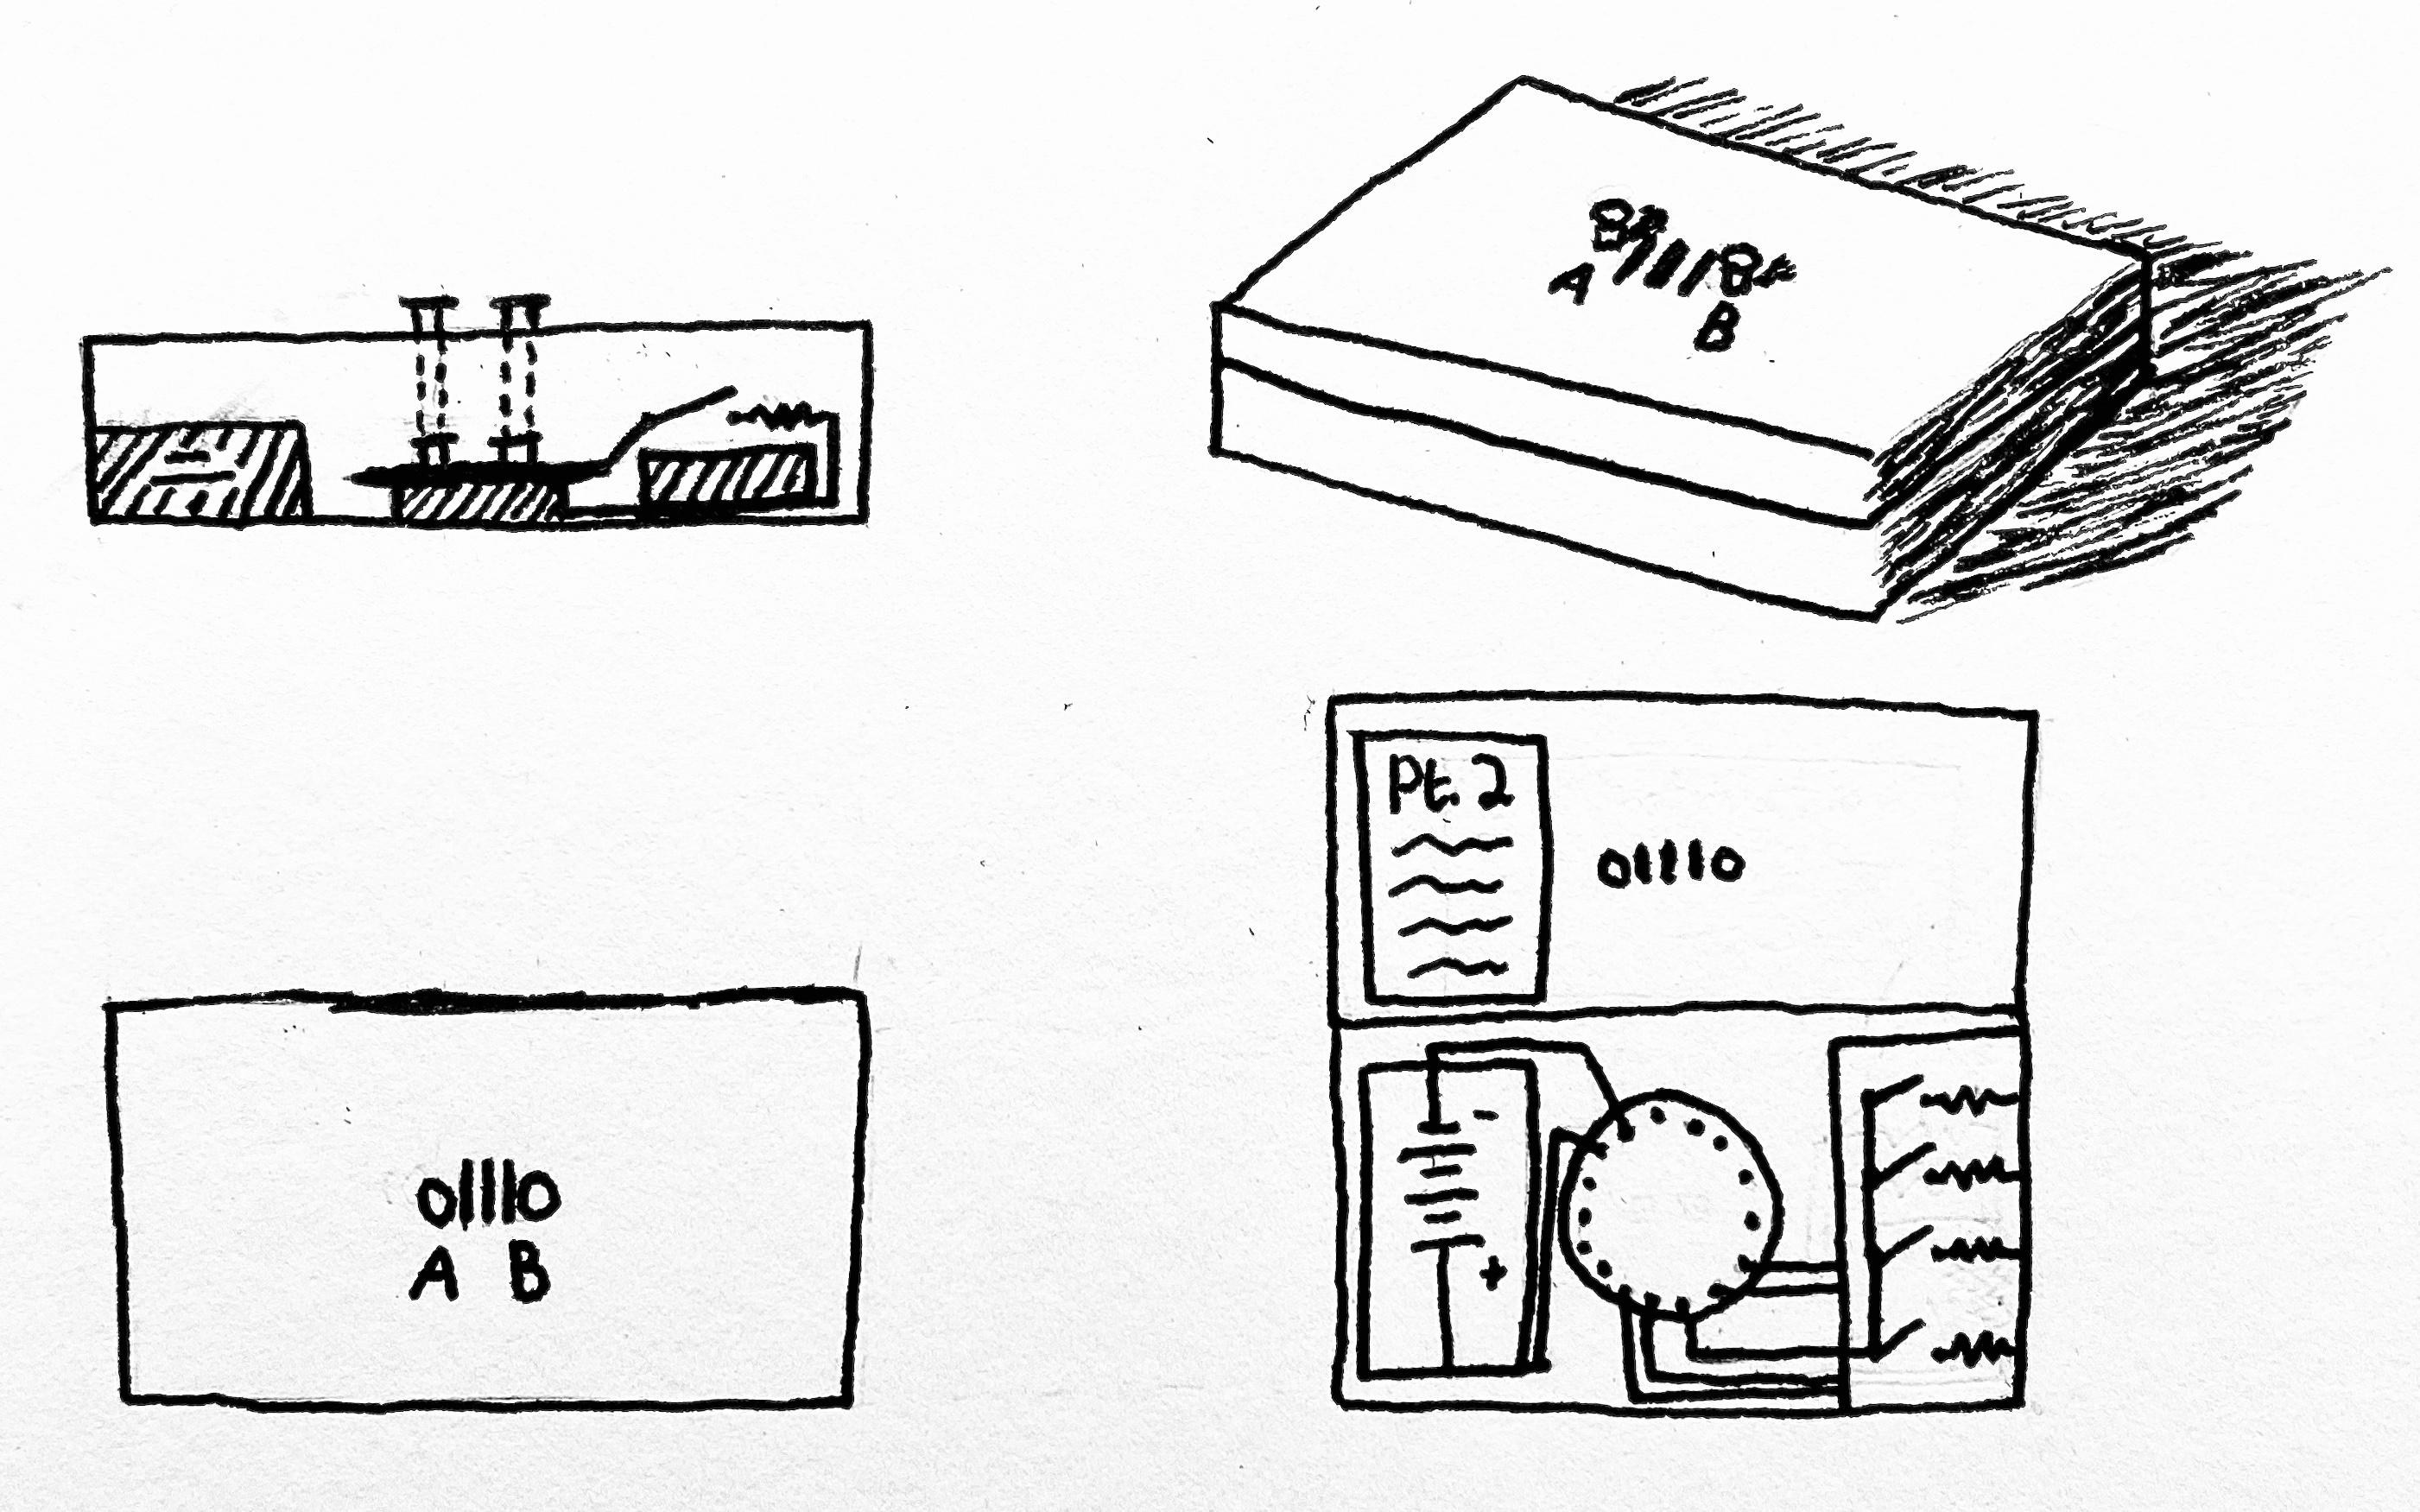
\includegraphics[width=4.5in]{IMG-2090.jpg}
    \caption{Concept Sketch of the Game}
    \label{fig:sketch}
\end{figure}

The final design for the outside of the game box with the toggles can be seen below in Figure \ref{fig:outside}.  The inside of the game box, which is used in the last two stages of the game, can be seen in Figure \ref{fig:inside}. 


\begin{figure}[ht!]
\centering
\begin{minipage}{.5\textwidth}
  \centering
  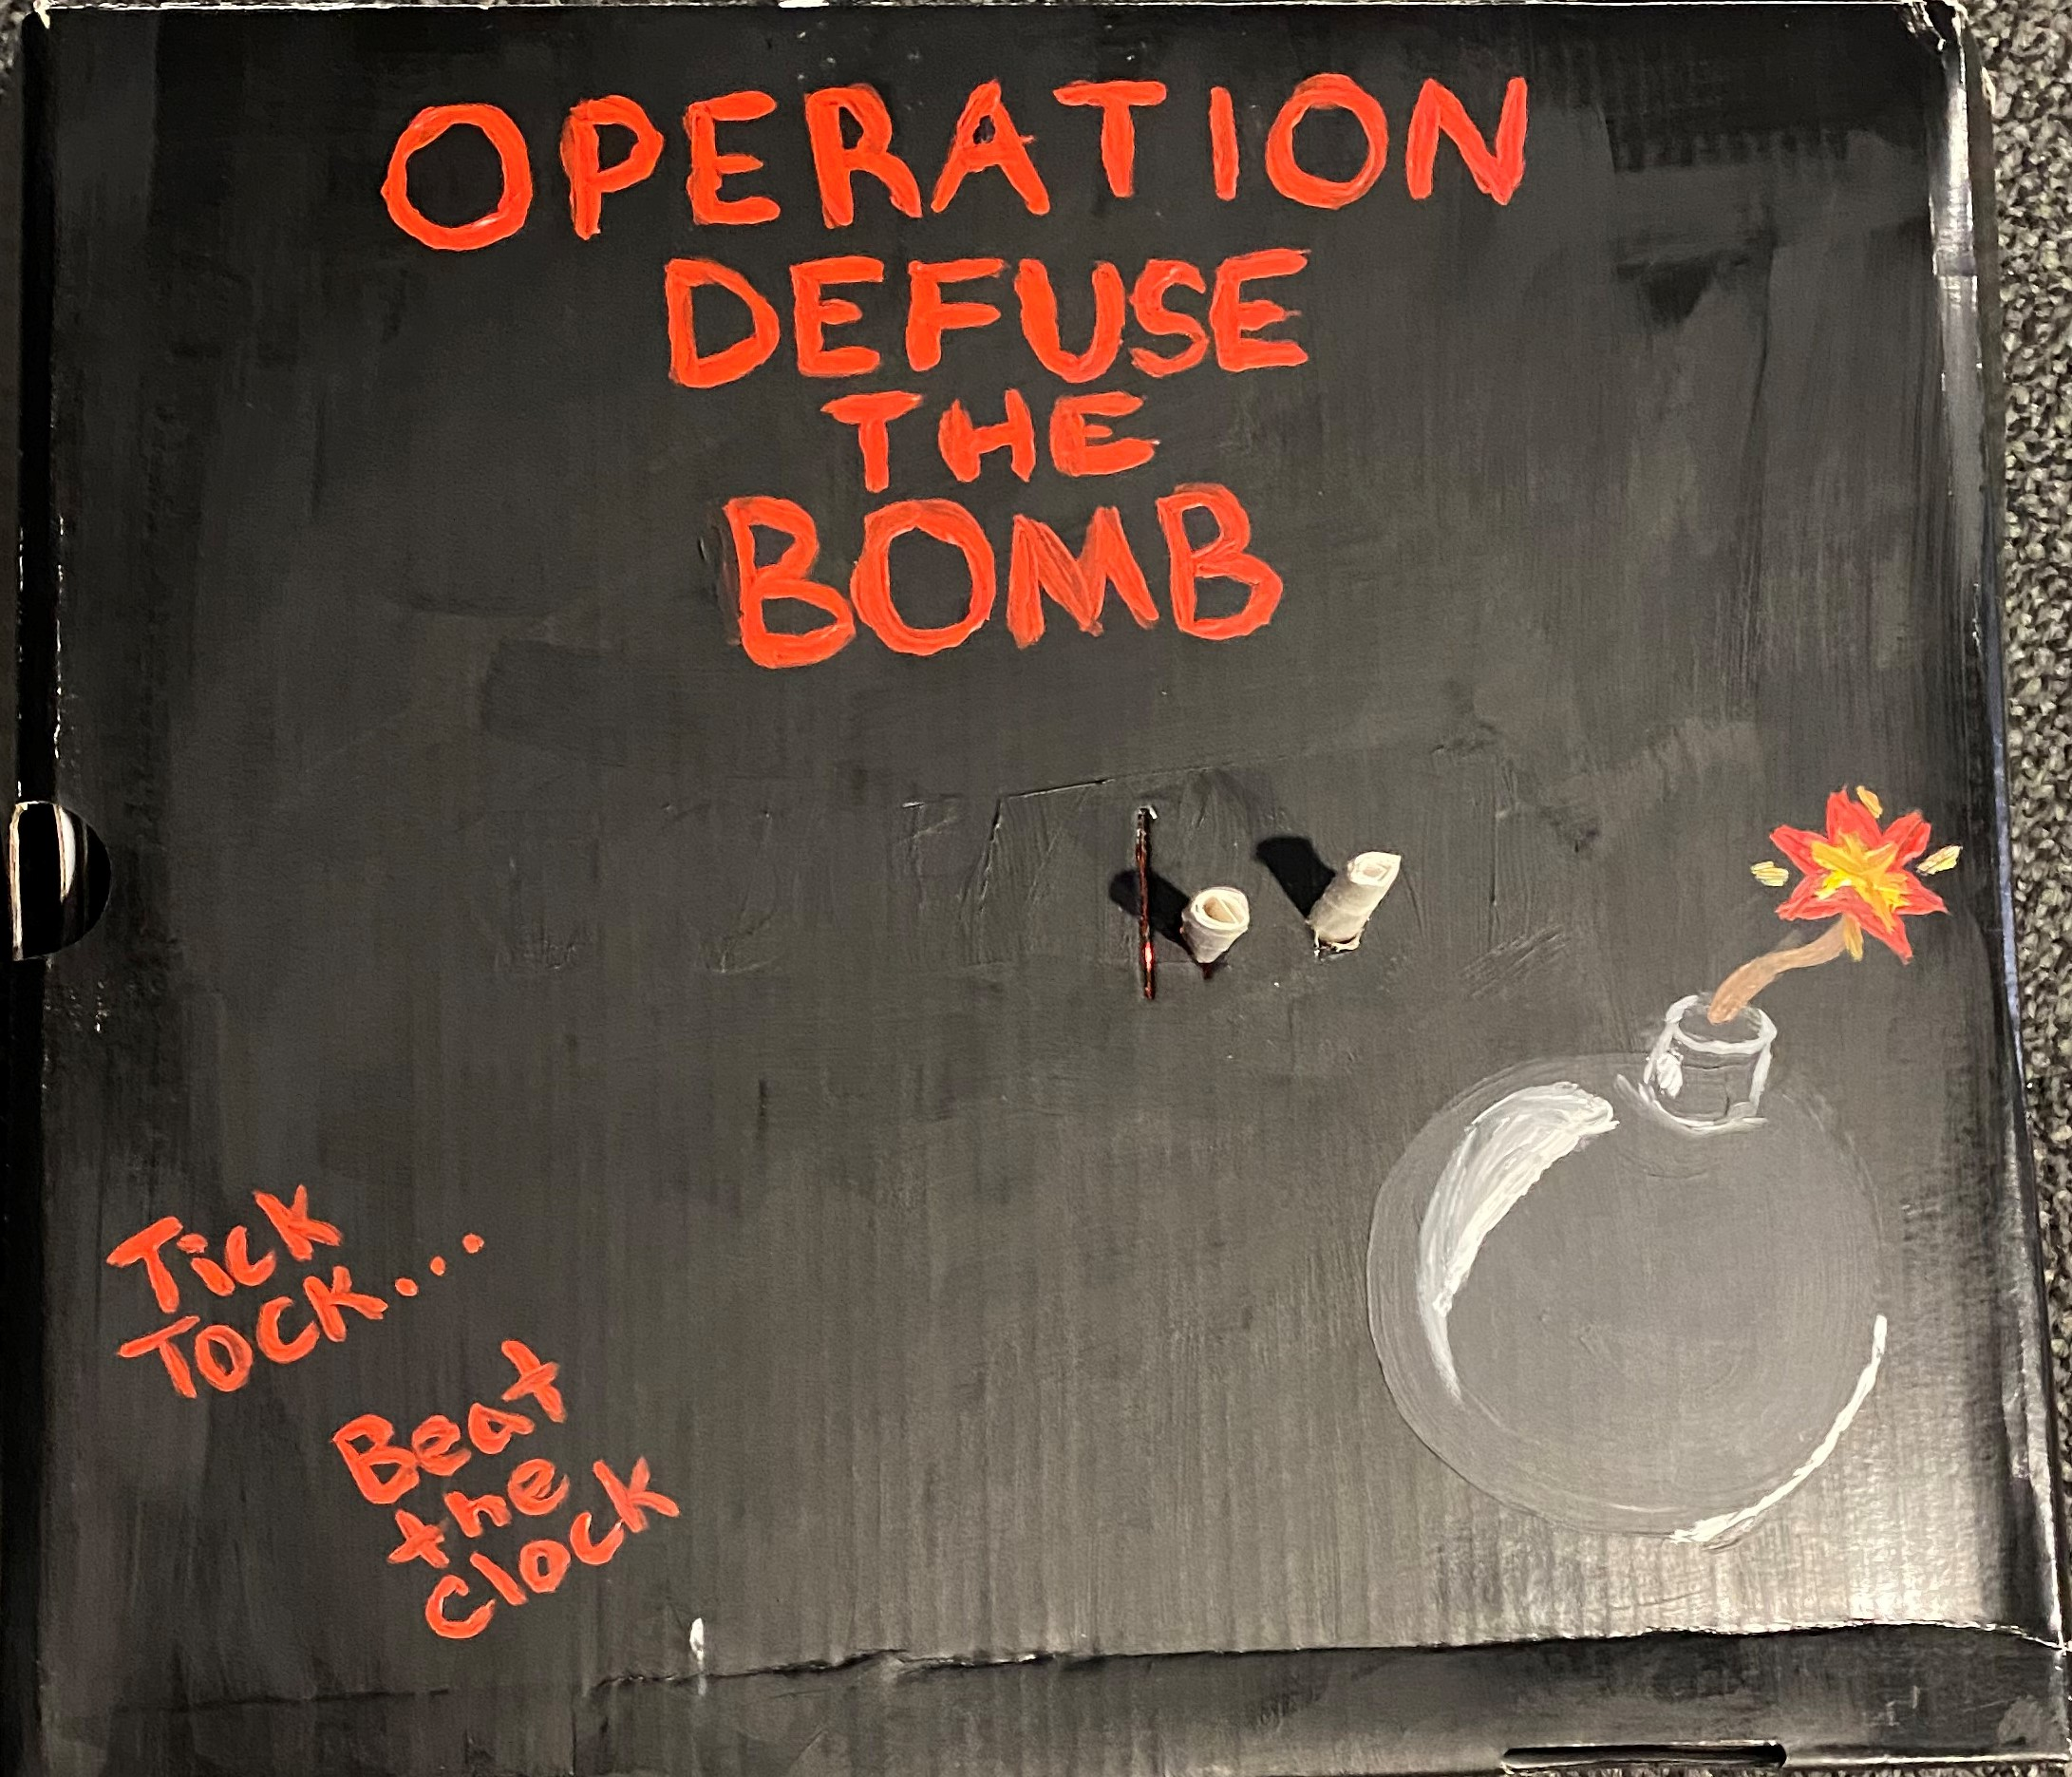
\includegraphics[width=2.9in]{img1.jpg}
  \caption{Outside of Game Box}
  \label{fig:outside}
\end{minipage}%
\begin{minipage}{.5\textwidth}
  \centering
  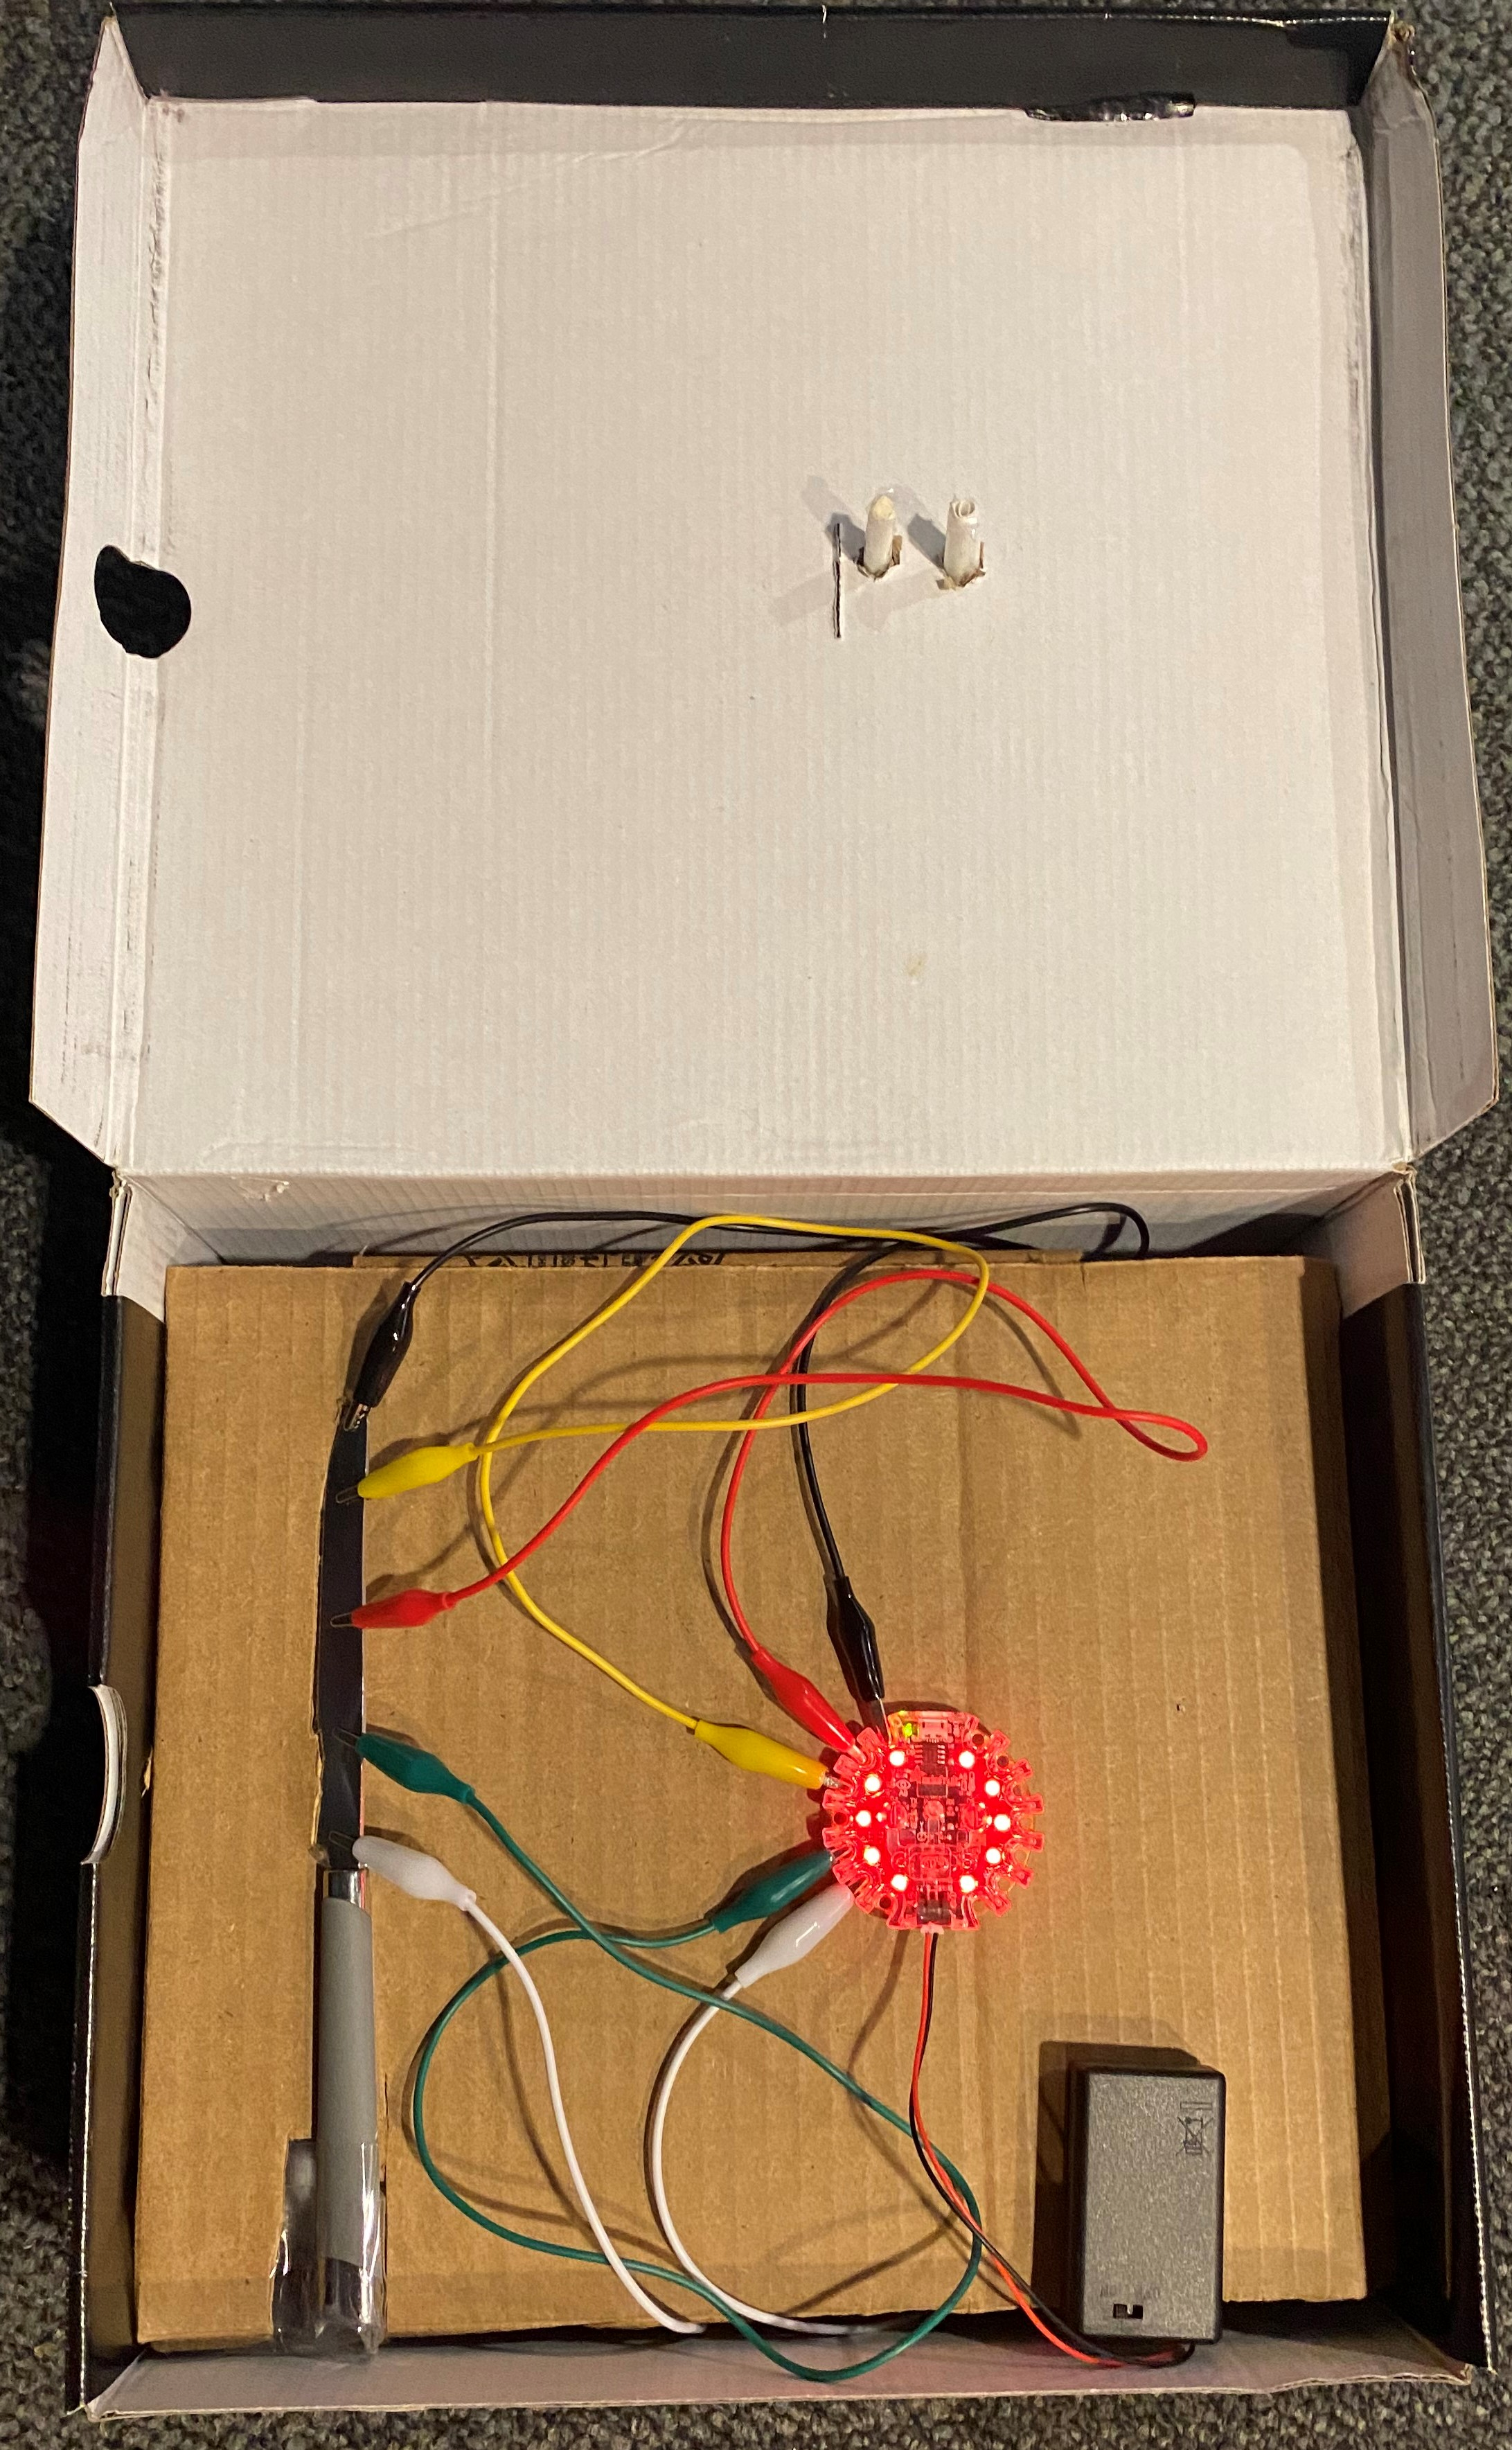
\includegraphics[width=2.9in]{img2.jpg}
  \caption{Inside of Game Box}
  \label{fig:inside}
\end{minipage}
\end{figure}
\newpage

\subsection{Game Play}

The following describes the final order of operations for the game play which features three pattern puzzles. First, the game is activated by sliding the switch on the power pack on.  There is then a small delay prior to the game starting to give the user time to close the box.  The game timer is started, and five blue neopixels light up and shut of incrementally, indicating the countdown.  Next, the user must unlock the box by listening for a high pitch and low pitch eight-tone pattern from the speaker and repeating it back.  The player can do so by using the left push button to repeat low tones and right push button to repeat high tones. During this sequence, the light sensor is active and the player will lose the game if the box is opened prior to correctly repeating the pattern.  After gaining access to the bomb inside the box, the player must push either of the push buttons to see the clip removal color sequence displayed on a single neopixel.  The clips and wires are connected from four of the capacitive touch pads, with one extra black wire and clip used for grounding, to the metal piece. The user must remove the clips from the from the metal piece in the correct color sequence (a butter knife was used for the prototype).  Either of the push buttons must be pressed again and the reattachment sequence is play.  Again, the player must attach the wires in the correct color sequence, and then the game is won! If the player completes all of the sequences without error and in the given time all of the neopixels will flash green indicating winning the game. 

\subsection{Program}
The program for this game was completed in different stages.  In the program setup, the following was defined: an initial state, an audio game, an open box state, and two wire games. A losing function was created to make the neopixels flash red if any of the stages of the game were lost such as incorrect pattern repeats, opening the box before the light sensor was turned off, or running out of time.  A similar function was created to flash green neopixels as the winning sequence. And lastly, a time loop was created for the time sequence of the game. 

The first stage of the game is the audio game. A loop is run to create an eight-value array with a random sequence of ones and zeros. If there is a one, a high tone is played, and a low tone is played for a zero. Moving on to the user input section, values of 0 and 1 were stored in an array based on the button pressed. The high tones are assigned to the B button, the low tones were assigned to the A button. A new loop checks to verify the input matches the tones played, and if they do not the bomb "detonates" and the losing sequence is run. 

Once the audio game is passed, the light sensor is deactivated and the player is allowed to open the box. After the user has access inside the box, the user then presses a button to receive a four color pattern, each color corresponding to one of the wires connected to the CPX. Much like the audio game, this is created using a random number generator, and the control flow is handled using a switch statement. In each case, the computer does nothing if the state of the wires remains the same. If the correct one is removed, the switch advances to the next case. If the wrong one is removed, the bomb goes off. As each wire is removed, the variable \texttt{wirestate} is advanced by one, which advances the cases, until they are all removed in the correct order.

If the player gets this far, and not many do, they must press another button to get another random pattern to reattach the wires. This is accomplished the same way as before with a random number generator, but saved in reverse. That way, we can use the same functions as before to check that the wires are being reattached in the correct order, but once again in reverse. All said and done, there are 5 functions for each possible state:
\begin{enumerate}
    \item All wires attached
    \item One wire removed
    \item Two wires removed
    \item Three Wires removed
    \item All wires removed
\end{enumerate}
Each of these functions take in the \texttt{order} vector, which contains the order of the input pins that each wires is connected to, which allows for all 24 possible patterns. After this, the bomb is defused, death is evaded and the game is won.

The source code for this project and a link to the GitHub repository used to complete this project can be found in Appendix A.

\section{STATUS}

This game was successfully completed, although there were some modifications to the original proposal.  The original proposal included a motion sensor that would have added a level of difficulty to the game by challenging the player to more carefully complete each stage of game play.  The motion sensor was excluded from the game due to difficulties in the level of sensitivity of the sensor.  With the external button presses using rolled Bristol and the removal and attachment of the alligator clips, it was decided to just eliminate this aspect of the game play.  Furthermore, the use of the slide switch to indicate completion of each stage was replaced with use of the push buttons.  Finally, the target audience age range was increased due to difficulty in the length of the patterns. 

\subsection{Challenges and Lessons Learned}
Multiple challenges were faced in completing the project.  Some of these challenges included the design of the box for the game, overcoming very little in-person interaction with distance learning, difficulties in utilizing a broad range of built-in functions, and creating the wires games.  Along with these challenges, there certainly were lessons learned along the way.

To begin with, the design of the box was a little bit tricky.  The biggest challenge with the box design was how to still utilize the push buttons.  Because we wanted to utilize the light sensor we needed to find a way to use the push buttons with the Circuit Playground Express board closed inside of the box. Although this wasn't ideal, we used rolled Bristol through holes in the lid of the box to create toggles to push the buttons.  The board was then taped down so that the buttons would be in the same place.

Next, overcoming a lack of in-person interaction was certainly a challenge.  Using phone apps and emails to interact without consistently scheduled meeting times made it more difficult to keep teammates updated with progress and challenges.  While there was no conflict in the team, we did face the challenge of having non-responsive teammates leading to a smaller group in the end.  To avoid some of these challenges in future projects, setting reoccurring meeting and messaging times to avoid procrastination and communication challenges should be implemented.

Furthermore, our proposal included the use of many of the built-in functions of the Circuit Playground Express.  This required reading and research on how each function and input and output pins worked and how to implement the use of each. To learn how to utilize .

Finally, the biggest challenge was creating the wires game.  The solution to creating the wires game was to set up wire states, similar to those found in \textit{How to Defuse a Time Bomb Game}. \cite{instructables-circuits}.  The wire game also used the capacitive touch pads.  To solve the challenge of completing that portion of the wire game, \textit{Circuit Playground Fruit Drums} was used as a reference for how to implement a capacity threshold and read the capacitive touch \cite{fruit-drums}.  The wire states can be seen below in Figure \ref{fig:wires}.

\begin{figure}[h!]
    \centering
    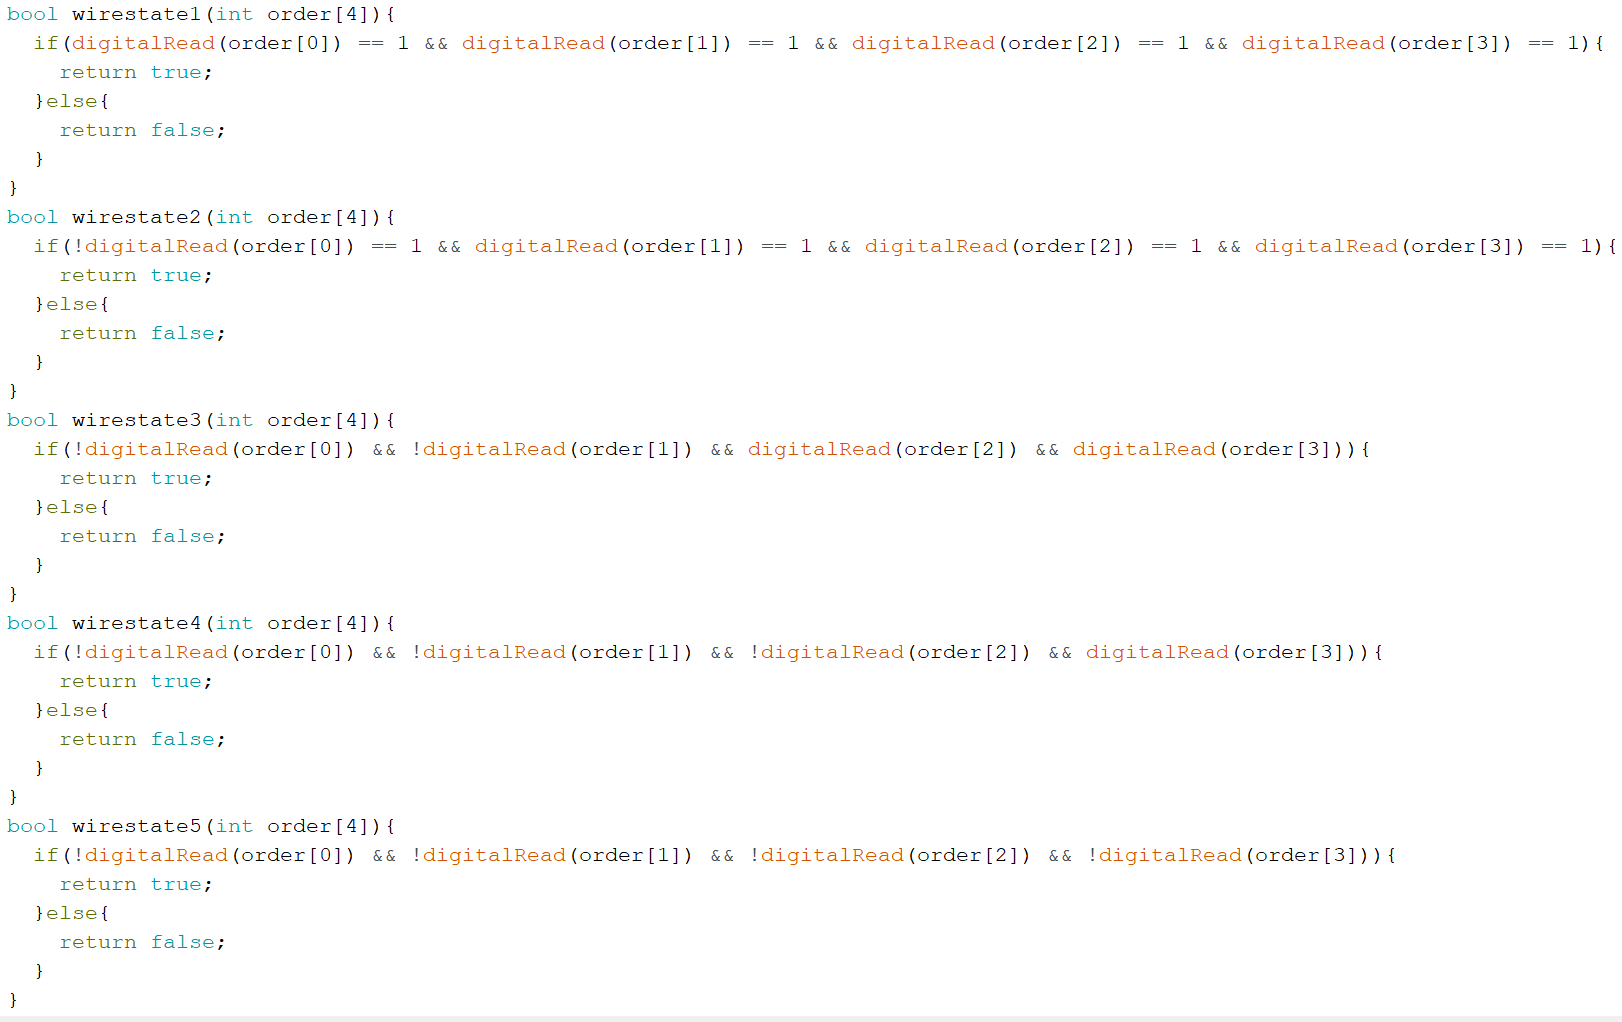
\includegraphics[width=4.5in]{wire states.PNG}
    \caption{Wire States}
    \label{fig:wires}
\end{figure}

Solutions to some of these challenges could have been better dealt with had we started the project by assigning sections of work, setting goal deadlines, and scheduling meetings at the beginning of the project.

\section{RESULTS}

Feedback and reactions from other students were collected to analyze the success of the game. The key points from the feedback are as follows:
\begin{enumerate}
    \item It can difficult to press the push buttons from outside of the box with the toggles
    \item The tone pattern is difficult to beat
    \item It would be useful to have different difficulty levels
    \item The game is a fun, but challenging
    \item The makeshift design of the game adds to the bomb simulation
\end{enumerate}

From this feedback we learned that while the game is a fun challenge, there is certainly room for improvement in our game.  Creating levels of difficulty would certainly be a great feature for this game. Furthermore, the design of of the game box could also use some improvements.  These issues are expanded upon below.

\section{FUTURE WORK}
There are two major areas that could use work to improve our design. First, the shoe box with rolled Bristol to press the buttons and a grounded butter knife for capacitance is a little jury-rigged to say the least. It is sufficient for a proof of concept, but of course not for a polished final product, so we would likely try to assemble a box and posts out of wood, and a purpose-made metal piece for connecting the wires.

Another good addition in the coding would be the creating multiple difficulty levels by modifying things such as the speed of audio and visual patterns, the overall time limit, and the capacitance limit, as a lower capacity makes the wires much more touchy and require more attention. In terms of the general purpose, this would allow for an even broader audience than any one fixed difficulty level.  This upgrade would cement the game's versatility as either a standalone game or an addition to a larger game such as an escape room or even a paintball version of \textit{Counterstrike}.

\section{CONCLUSION}

In conclusion, Team CYclones Git Solutions saw an opening in the game market and found a solution to this problem by brainstorming ideas to create an entertaining game. Once the team decided upon \textit{Operation: Defuse the Bomb}, key features were decided upon, and an algorithm was then written to help plan the program. \textit{Operation: Defuse the Bomb} is a stimulating game that simulates defusing a bomb by utilizing many of the built-in functions of the Circuit Playground Express including the mini neopixels, light sensor, mini speaker, push buttons, capacitive touch pads, and alligator clips.  After deciding how the game should be played, the program was completed with three mini-game stages including repeating tone patterns and removing and reattaching the alligator clips in a given light pattern.  Throughout the process of creating this game, the team faced and overcame challenges through which a few key lessons were learned.  After the initial design, the game was refined to remove the use of the motion sensor, alter the design of the game box, and modify the target audience range.  By gathering feedback, the team concluded that the box design and difficulty levels could be improved upon in future versions.  All in all, the \textit{Operation: Defuse the Bomb} project was a success.

\newpage

\bibliographystyle{plain}
\bibliography{ref}
\newpage
% you need to have at least your code in your appendix
\appendix

\section{SOURCE CODE}
The following is the link to the team GitHub repository: \url{https://github.com/AerE-361-FinalProject/CYGS} \\
\\
Source Code
\lstinputlisting[language=Arduino]{timebomb_main.ino}
\end{document}
